%%%%%%%%%%%%%%%%%%%%%%%%%%%%%%%%%%%%%%%%%
% Daily Laboratory Book
% LaTeX Template
% Version 1.0 (4/4/12)
%
% This template has been downloaded from:
% http://www.LaTeXTemplates.com
%
% Original author:
% Frank Kuster (http://www.ctan.org/tex-archive/macros/latex/contrib/labbook/)
%
% Important note:
% This template requires the labbook.cls file to be in the same directory as the
% .tex file. The labbook.cls file provides the necessary structure to create the
% lab book.
%
% The \lipsum[#] commands throughout this template generate dummy text
% to fill the template out. These commands should all be removed when
% writing lab book content.
%
% HOW TO USE THIS TEMPLATE
% Each day in the lab consists of three main things:
%
% 1. LABDAY: The first thing to put is the \labday{} command with a date in
% curly brackets, this will make a new page and put the date in big letters
% at the top.
%
% 2. EXPERIMENT: Next you need to specify what experiment(s) you are
% working on with an \experiment{} command with the experiment shorthand
% in the curly brackets. The experiment shorthand is defined in the
% 'DEFINITION OF EXPERIMENTS' section below, this means you can
% say \experiment{pcr} and the actual text written to the PDF will be what
% you set the 'pcr' experiment to be. If the experiment is a one off, you can
% just write it in the bracket without creating a shorthand. Note: if you don't
% want to have an experiment, just leave this out and it won't be printed.
%
% 3. CONTENT: Following the experiment is the content, i.e. what progress
% you made on the experiment that day.
%
%%%%%%%%%%%%%%%%%%%%%%%%%%%%%%%%%%%%%%%%%

%----------------------------------------------------------------------------------------
%	PACKAGES AND OTHER DOCUMENT CONFIGURATIONS
%----------------------------------------------------------------------------------------

\documentclass[idxtotoc,hyperref,openany]{labbook} % 'openany' here removes the gap page between days, erase it to restore this gap; 'oneside' can also be added to remove the shift that odd pages have to the right for easier reading


\usepackage[
  backref=page,
  pdfpagelabels=true,
  plainpages=false,
  colorlinks=true,
  bookmarks=true,
  pdfview=FitB]{hyperref} % Required for the hyperlinks within the PDF

\usepackage{booktabs} % Required for the top and bottom rules in the table
\usepackage{float} % Required for specifying the exact location of a figure or table
\usepackage{graphicx} % Required for including images2
\usepackage{lipsum} % Used for inserting dummy 'Lorem ipsum' text into the template

% The following packages can be found on http:\\www.ctan.org
%\usepackage{graphics} % for pdf, bitmapped graphics files
\usepackage{epsfig} % for postscript graphics files
%\usepackage{mathptmx} % assumes new font selection scheme installed
%\usepackage{times} % assumes new font selection scheme installed
\usepackage{amsmath} % assumes amsmath package installed % aligned
\usepackage{amssymb}  % assumes amsmath package installed

% This adjusts the underline to be in keeping with word processors.
\usepackage{color}
\usepackage{soul}
\setul{.6pt}{.4pt}
\setulcolor{red}
\setstcolor{green}
\sethlcolor{yellow}

\usepackage{verbatim}

\newcommand{\HRule}{\rule{\linewidth}{0.5mm}} % Command to make the lines in the title page
\setlength\parindent{0pt} % Removes all indentation from paragraphs

%----------------------------------------------------------------------------------------
%	DEFINITION OF EXPERIMENTS
%----------------------------------------------------------------------------------------

\newexperiment{example}{This is an example experiment}
\newexperiment{example2}{This is another example experiment}
\newexperiment{example3}{This is yet another example experiment}
\newexperiment{table}{This shows a sample table}
%\newexperiment{shorthand}{Description of the experiment}

\newexperiment{item1}{Tasks I completed today:}
\newexperiment{item2}{Tasks I could not complete today, and why:}
\newexperiment{item3}{Reflections}
\newexperiment{item4}{What do I want to achieve tomorrow:}

%---------------------------------------------------------------------------------------

\newtheorem{theorem}{Theorem}
\newtheorem{definition}{Definition}
\newtheorem{lemma}{Lemma}
%\newtheorem{proof}{Proof}
\newtheorem{remark}{Remark}
\newtheorem{assumption}{Assumption}

\begin{document}

%----------------------------------------------------------------------------------------
%	TITLE PAGE
%----------------------------------------------------------------------------------------

\frontmatter % Use Roman numerals for page numbers
\title{
\begin{center}
\HRule \\[0.4cm]
{\Huge \bfseries Online Lectures \\[0.5cm] \Large Division of Electrical Engineering & Computer Engineering, Louisiana State University and Agricultural and Mechanical College
}\\[0.4cm] % Degree
\HRule \\[1.5cm]
\end{center}
}
\author{\Huge Shaopan Guo \\ \\ \LARGE gshaop1@lsu.edu \\[2cm]} % Your name and email address
\date{Beginning 15 August 2019} % Beginning date
\maketitle

\tableofcontents

\mainmatter % Use Arabic numerals for page numbers

%----------------------------------------------------------------------------------------
%	LAB BOOK CONTENTS
%----------------------------------------------------------------------------------------

% Blank template to use for new days:

%\labday{Day, Date Month Year}

%\experiment{}

%Text

%-----------------------------------------

%\experiment{}

%Text

%----------------------------------------------------------------------------------------

\labday{Long Actuator Delays - Extending the Smith Predictor to Nonlinear}

\section{Basic Information}

Long Actuator Delays - Extending the Smith Predictor to Nonlinear

Miroslav Krstic

Mechanical and Aerospace Engineering

University of California, San Diego

Abstract:
One would be hard pressed to find  "long actuator delays, "unknown delays," or "nonlinear control" co-existing in the same sentence in the control literature. This is due to the potential for finite escape in the presence of nonlinearity, and due to the uncertainty in the size of the infinite-dimensional part of the system's state in the case of unknown delay. It has been half a century since Otto Smith, a professor of Mechanical Engineering at UC Berkeley, invented the "predictor" feedback for compensating long but known actuator delays for linear systems. This method has since become one of the favorite tools in chemical process control and many other applications.  I will show an extension of predictor feedback to nonlinear (possibly unstable) systems, which is enabled by "infinite dimensional/continuum backstepping." Backstepping yields the construction of Lyapunov-Krasovskii functional with which I have been able to prove robustness of predictor feedbacks to both underestimating and overestimating the length of the actuator delay, as well as to develop the first delay-adaptive controllers.

Bio:
Miroslav Krstic is the Sorenson Professor of Mechanical and Aerospace Engineering and the Director of the newly formed Center for Control Systems and Dynamics (CCSD) at the University of California at San Diego. He is a coauthor of the books Nonlinear and Adaptive Control Design, Stabilization of Nonlinear Uncertain Systems, Flow Control by Feedback, Real Time Optimization by Extremum Seeking Control, and Control of Turbulent and Magnetohydrodynamic Channel Flows. Dr. Krstic received the National Science Foundation Career, ONR YI, and PECASE Awards, as well as the Axelby and the Schuck paper prizes. In 2005, he was the first engineering professor to receive the UCSD Award for Research. He is a Fellow of IEEE, a Distinguished Lecturer of the Control Systems Society, and a former CSS VP for Technical Activities.

Youtube video link: https://youtu.be/0Nt1Pf5H3rA

In the first two bullets, I will offer you some of the basic ideas for linear systems and show how a perspective on predictor base feedback using the infinite dimensional backstepping tools for partial differential equations can help establish stability and robustness properties for linear problems.

Then I will talk about an extension to predictor design for systems that have a delay on the other end, the sensor end.

Then I will talk about extensions to nonlinear systems and extensions to problems for the delays unknown long and needs to be estimated in a feedback loop.

And finally I will talk about some extensions of the predictor based ideas to actually dynamics and or plant dynamics that might be some other types of partial differential equations rather than the transport PD or delay.

And finally I will talk about a new subject that is linked to control PDEs in robotic swarming or coordinated motion control.

\section{Smith predictor as a form of infinite-dimensional 'backstepping'}

Delay systems are arising in many applications.

\subsection{Basic Observations}

\begin{itemize}
  \item thousands of papers and dozens of books since the 1940's (Tsypkin 1946)
  \item "golden era" = 1970's and early 1980's (Kalman, Sontag, Morse, Mitter, Artstein, Khargonekar, Tannenbaum)
  \item another "burst" of research activity after the introduction of LMIs (1990s)
  \item many basic problems still unsolved, till very active area of Research
  \item \hl{delay systems are infinite dimensional}
  \item \hl{the state is not a vector but a function (or a vector of functions); characteristic equation not a polynomial, involves exponentials}
  \item \hl{stability analysis requires Krasovskii functionals, rather than Lyapunov functions}
\end{itemize}

\subsection{Benchmark Delay System (Scalar)}

\begin{equation}
\dot{X}(t) = X(t-D) + U(t)~(\mathbf{easy},~cancel~or~dominate~by~high~gain)
\end{equation} $X$ is a scalar variable, $U$ is a control. When $D$ is zero, this is an unstable system \hl{(Why?)}. When the delay is nonzero this is a very easy problem. You can either cancel this destabilizing term using the measurement of the past value of the measured state $X$ or you can actually dominate using high gain. You do not have to exactly cancel it.

The next problem involves the delay on the input.

\begin{equation}
\dot{X}(t) = X(t) + U(t-D),~(\mathbf{hard},~need~inf.~dim.~controller~for~large~D)
\end{equation} That is a totally different problem. That is a problem that the Smith predictor and various other extensions deal with. That can be a very hard problem and I will talk about that one.

The one I will not talk about is a problem that involves simultaneous delay on state and control.

\begin{equation}
\dot{X}(t) = X(t-D_1) + U(t-D_2),~(\mathbf{even~harder},~conceltually)
\end{equation} Even when the state $X$ is scalar valued this can be a pretty hard problem \hl{particularly if the delay on the input is longer than the delay on the state.} And in the vector case it is essentially unsold at the moment\footnote{This presentation was published twelve years ago. Is there any progress in the recent years?}. So I would focus on the second of the three problems.

\subsection{Actuator delaycompensation by Backstepping}

So I have to admit that before getting into delay systems I had not learned this problems gradually. I knew close to nothing. I was working on control of OPDs and even did not think that what I was doing whould apply to delay systems. Simply because the results that I had up until that time were for pds involving at least two derivatives in space whereas the delay involves only one derivative only a convective effect. So I tried once and here is how this went this experience of mine I think it is actually very usefull one can learn something and get excited about it. So let me now consider a vector problems for a full general linear controllable system with delay on the input.

\begin{equation}
\dot{X}(t) = AX(t) + BU(t-D).
\end{equation} Let me assume that the pair $(A, B)$ is controllabel and let me assume that I have picked some nominal control case to stabilize the undelyed system. And now let me go ahead and replace the simple delay notation with a PD representation.So let me represent delay subsystem using a transport equation. So this transport equation is given here this PD.

A transport PDE representation:

\begin{equation}
  \begin{aligned}
      \dot{X}(t) &= AX(t) + Bu(0,t)\\
      u_t(x,t) &= u_x(x,t)\\
      u(D,t) &= U(t)
  \end{aligned}
\end{equation} The output of the transport equation is the delayed input and the boundary input into this transport PD is the actual control.

\begin{figure}[ht!]
\centering
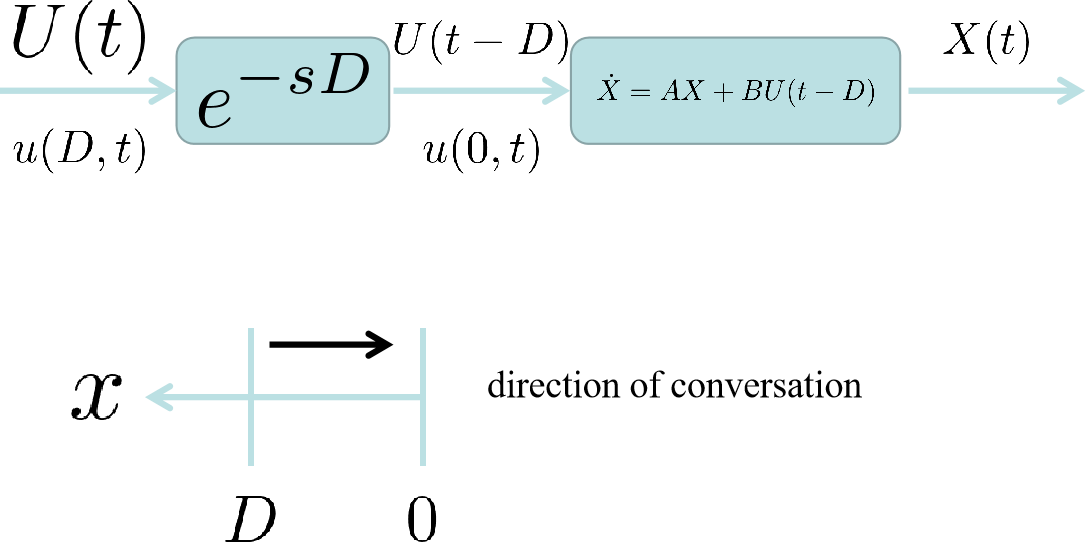
\includegraphics[width=0.9\textwidth]{figure_1.png}
%\caption{A platoon consisting of $N$ vehicles}\label{Illustration_v2}
\end{figure} So this is a very particular PD, sort of simpplest of PDs, and it can actually be solved in closed form if the input is given.

SO here is how the so-called backstepping method for PD goes.

\bf{Consider the backstepping transformation}

\begin{equation}
  w(x,t) = u(x,t) - \int_0^x q(x,y)u(y,t)dy - \gamma(x)^T X(t)
\end{equation}

By the way why think this problem is a PD problem. Well, because it is a boundary control problem I have a cascade of a partial differential equation $u$ with an OD $X$ and the input enters at the boundary $X$ equal to $D$ of this PD. So comming from that background this is how you formulate this problem and given that there are tools for boundary controlling the in the context of this continue or infinite backstepping this is how you approach this problem. You approach it by constructing an infinite dimensional transformation a continuum transformation of the actuator state $u$ into your new state $w$. This transformation I wil tell you in a second what its purpose is but its structure is a voltaire of transformation. So this integral in $y$ in the position $y$ runs from $0$ to the current $X$. So it is a lower triangular continuum operator so to speak. There is also the OD part in this transformation which is crucial so here's the objective

\bf{and the target system}

\begin{equation}
    \begin{aligned}
        \dot{X}(t) &= (A + BK)X(t) + Bw(0,t)\\
        x_t(x,t) &= w_x(x,t)\\
        w(D,t) &= 0.
    \end{aligned}
\end{equation} One wants to transform the original system into this traget system using that transformation one wants the transformation to be invertible.


\section{Robustness consequences}

\section{Observer design with sensor delay}

\section{Predictor feedback for nonlinear systems}

\section{Delay-adaptive control}

\section{Bonus 1: Other forms of infinite-dimensional actuator dynamics}

\section{Bonus 2: Robotic swarm choreography via PDE boundary control techniques}






%	FORMULAE AND MEDIA RECIPES
%----------------------------------------------------------------------------------------

\labday{} % We don't want a date here so we make the labday blank

\begin{center}
\HRule \\[0.4cm]
{\huge \textbf{Formulae and Media Recipes}}\\[0.4cm] % Heading
\HRule \\[1.5cm]
\end{center}

%----------------------------------------------------------------------------------------
%	MEDIA RECIPES
%----------------------------------------------------------------------------------------

\newpage

\huge \textbf{Media} \\ \\

\normalsize \textbf{Media 1}\\
\begin{table}[H]
\begin{tabular}{l l l}
\toprule
\textbf{Compound} & \textbf{1L} & \textbf{0.5L}\\
\toprule
Compound 1 & 10g & 5g\\
Compound 2 & 20g & 10g\\
\bottomrule
\end{tabular}
\caption{Ingredients in Media 1.}
\label{tab:med1}
\end{table}

%-----------------------------------------

%\textbf{Media 2}\\ \\

%Description

%----------------------------------------------------------------------------------------
%	FORMULAE
%----------------------------------------------------------------------------------------

\newpage

\huge \textbf{Formulae} \\ \\

\normalsize \textbf{Formula 1 - Pythagorean theorem}\\ \\
$a^2 + b^2 = c^2$\\ \\

%-----------------------------------------

%\textbf{Formula X - Description}\\ \\

%Formula

%----------------------------------------------------------------------------------------

\bibliographystyle{ieeetr}
\bibliography{shaopanguo_ref}

\end{document}
